\section{Project Plan}
\label{sec:projectplan}
For the planning of the project, I decided to use my experience from my 6-month placement to use more traditional software development methodologies,
making use of a Kanban board to track the progress of the project.

In this Kanban board, I have made use of labels to categorise each task into different categories, allowing me to make use
of the filter function to view tasks of a specific category.

\begin{figure*}[t]
  \begin{minipage}[t]{0.49\textwidth}
    \centering
    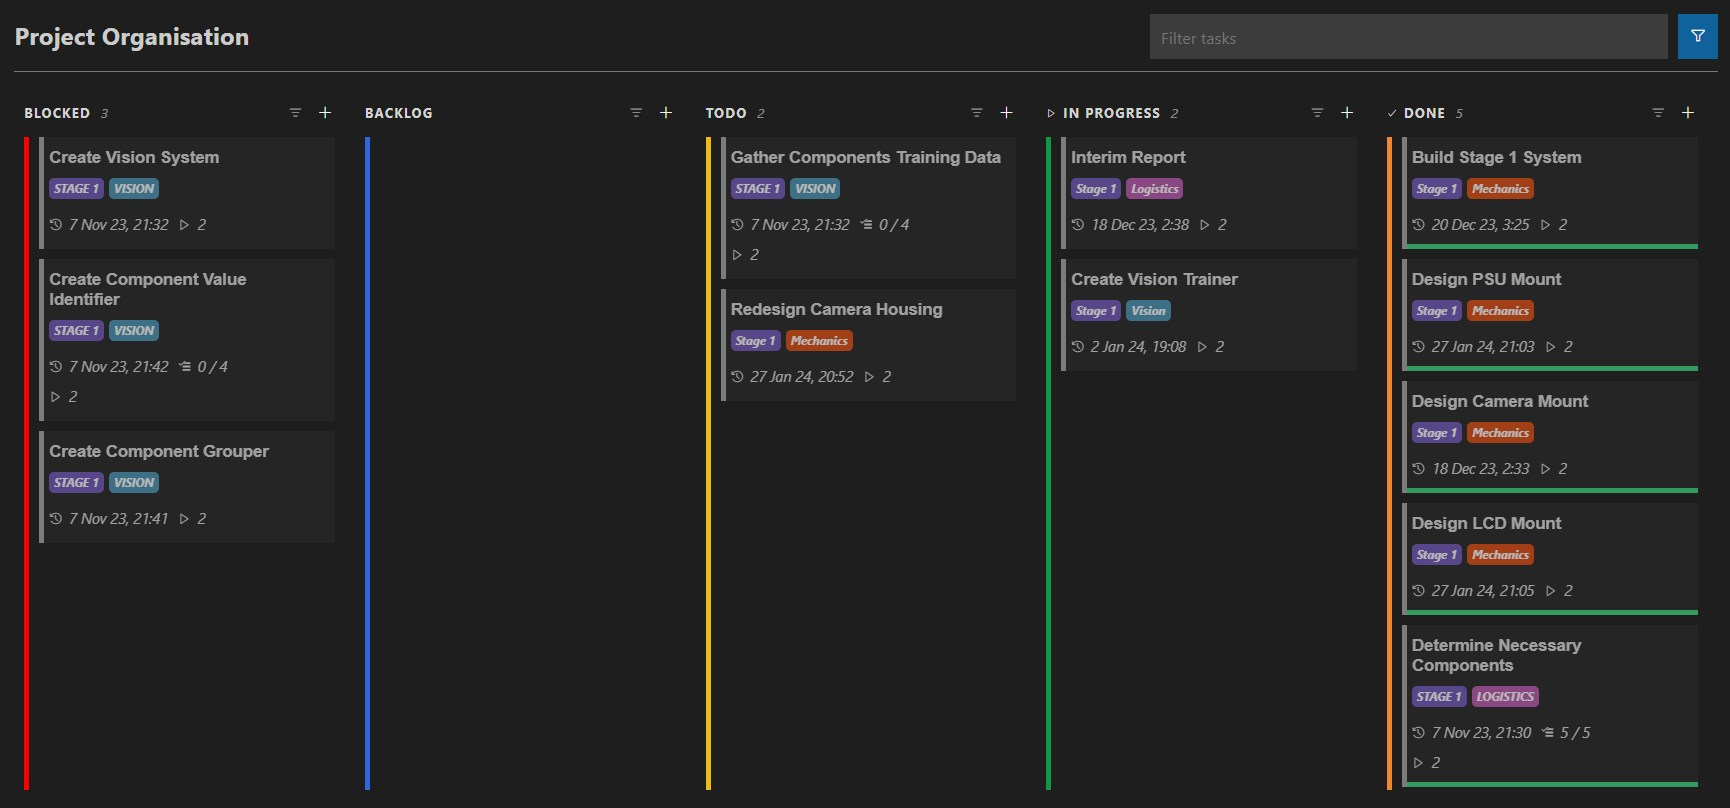
\includegraphics[width=\textwidth,height=4.5cm]{imgs/software/projectplan.jpg}
    \caption{Project Plan}
  \end{minipage}
  \hfill 
  \begin{minipage}[t]{0.49\textwidth}
      \centering
      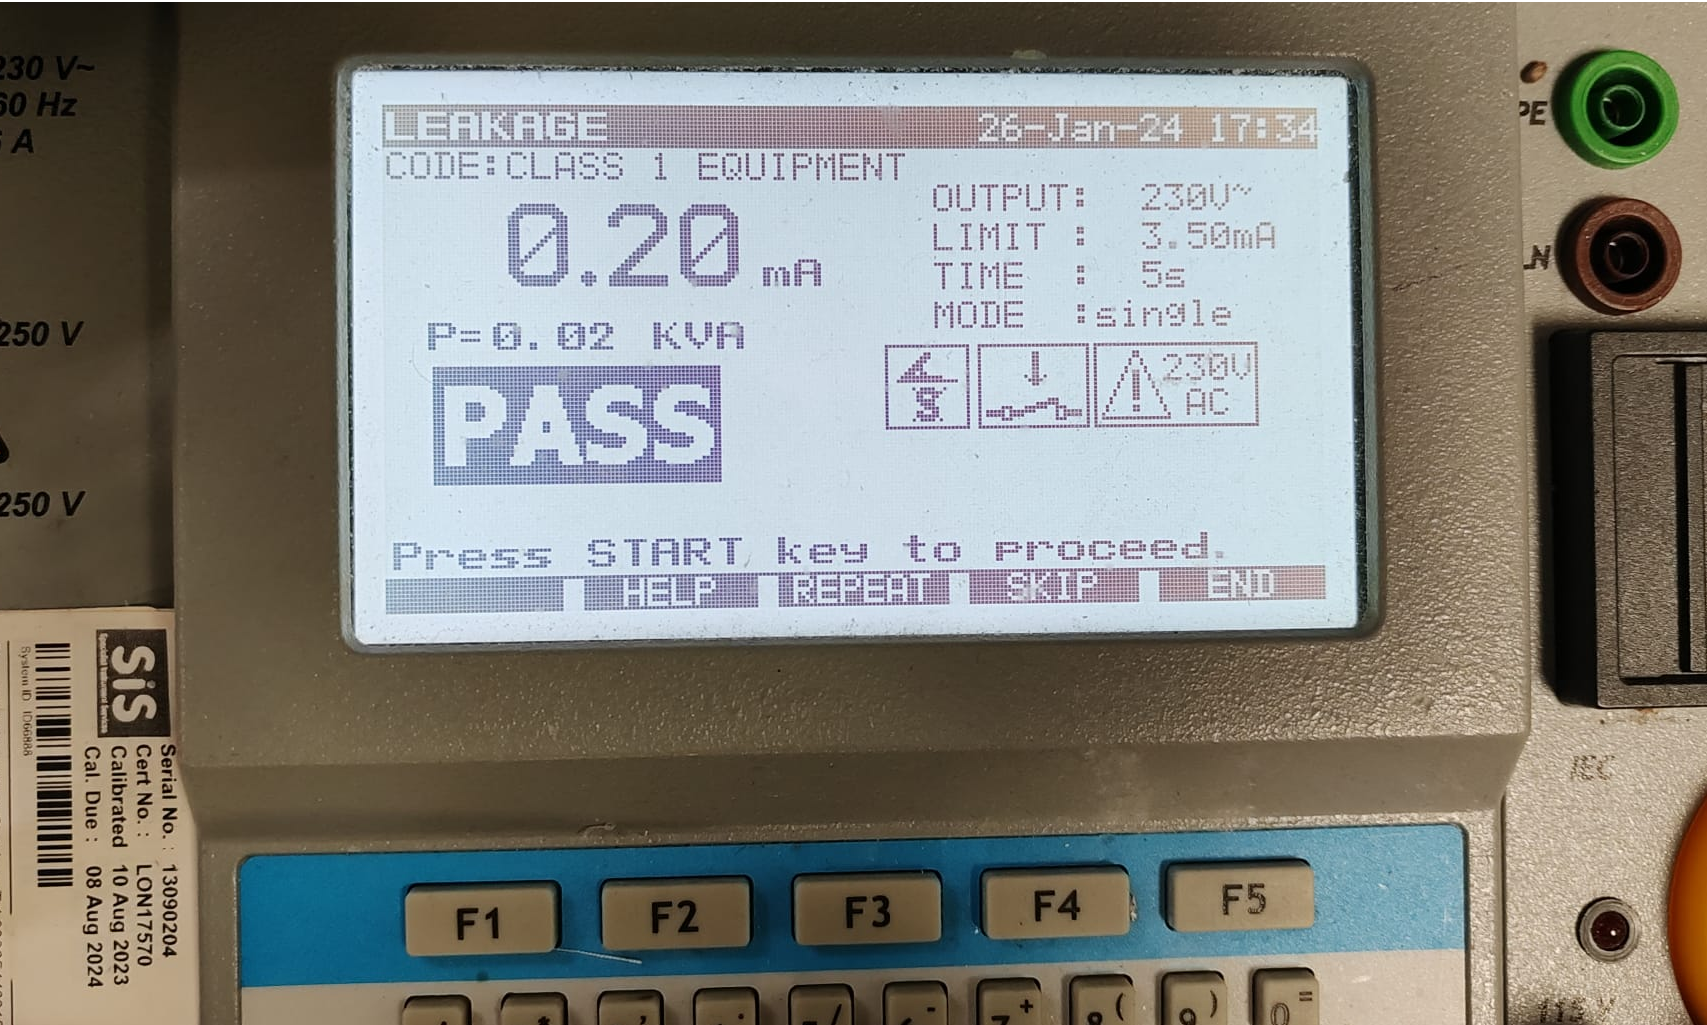
\includegraphics[width=\textwidth,height=4.5cm]{imgs/pattesting.jpeg}
      \caption{PAT Testing Results}
      \label{fig:pat}
    \end{minipage}
    \hfill
\end{figure*}

For the remainder of the project, I will be using this Kanban board to track the progress of the project. 
 \subsection{Stage 1}
The Stage 1 system is not currently complete, however, I have made significant progress towards the completion of the system. The remaining
tasks for the Stage 1 system are to redesign the camera mount so that it is down-facing, collect training data for the Stage 1 system, and
train the component detection model. 

While non-trivial, I believe that these tasks can be completed within the next 3 weeks due to the strong foundation of the project, allowing me to move onto the Stage 2 system.
The current Stage 1 system is shown in Figure \ref*{fig:allparts}.

\subsection{Stage 2}
For the Stage 2 system, the system will become semi-autonomous, with the user having to manually place the components into the system, and the system
automatically sorting the components into the correct bins after classifying and identifying the components. 

For the Stage 2 system, the following tasks will need to be completed:
\begin{mylist}
    \item \textbf{Component Value Identification} \\
    After the component has been classified, the system will need to identify the value of the component. This will be done by using
    a separate model to identify the value of the component. In particular, the model for the resistors will be the highest
    priority given their complexity, followed by text-based values for capacitors and inductors, and finally ICs and MOSFETs.
    \item \textbf{Conveyor Belt System} \\
    The system will need to be able to move the components from the camera to the sorting mechanism. This will be done using a conveyor belt system
    that will be controlled by the Raspberry Pi.
    \item \textbf{Sorting Mechanism} \\
    The system will need to be able to sort the components into the correct bins. This will be done using a servo motor to move the components into the correct bin.
    This not only requires the software to be developed but also the physical mechanism to be designed and built, including the bins themselves.
    \item \textbf{User Interface} \\
    The UI of the system will need to be updated to reflect the system's new functionality. This will be done using the Pygame library\cite{pygamedoc}.
\end{mylist}

\noindent
In terms of time management, I am only taking 2 modules this term, as I decided to take 4 modules in the first term. Substantial work has already been completed
during the Christmas break, so I am confident that I will be able to spend sufficient time on the project during this term.

\subsection{Stage 3}
The final stage of the system will be to make the system fully autonomous, with the system being able to identify and sort components without any user input.
The main task for this stage will be to develop a device that can automatically feed the components into the system, and as 
discussed in Section \ref*{sec:background} (Background), this will likely be done with a vibratory bowl feeder (VBF).

Ensuring system reliability will also be a key task for this stage, as at this point the system will contain many moving parts, and will need to be able to
operate reliably for extended periods. I expect that this stage will most involve fine-tuning the system and doing logistics such as
finalising the report and presentation.